244. \begin{figure}[ht!]
\center{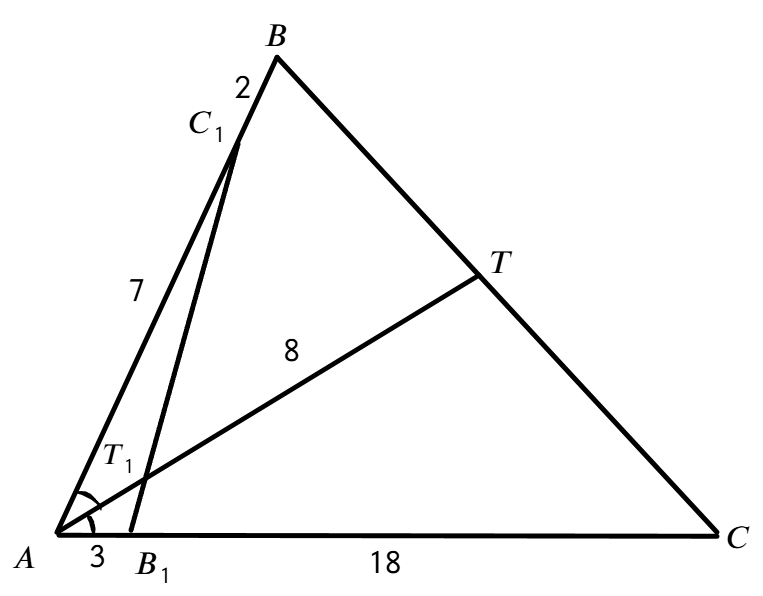
\includegraphics[scale=0.35]{g8-241.png}}
\end{figure}\\
Найдём $AB=AC_1+C_1B=2+7=9$ и $AC=AB_1+B_1C=3+18=21.$ Треугольники $ABC$ и $AB_1C_1$ подобны по первому признаку: $\cfrac{AB}{AB_1}=\cfrac{AC}{AC_1}=3,$ угол $A$ --- общий. Тогда с тем же коэффициентом подобия относятся друг к другу и их биссектрисы: $\cfrac{AT}{AT_1}=3,\ \cfrac{AT_1+8}{AT_1}=3,\ 2AT_1=8,\ AT_1=4.$\\
